%%%%%%%%%%%%%%%%%%%%%%%%%%%%%%%%%%%%%%%%%%%%%%%%%%%%%%%%%%%%%%%%%%%%%%%%%%%
%% This file is part of the book
%%
%% Algorithmic Graph Theory
%% http://code.google.com/p/graph-theory-algorithms-book/
%%
%% Copyright (C) 2009, 2010, 2011 Minh Van Nguyen <nguyenminh2@gmail.com>
%%
%% See the file COPYING for copying conditions.
%%%%%%%%%%%%%%%%%%%%%%%%%%%%%%%%%%%%%%%%%%%%%%%%%%%%%%%%%%%%%%%%%%%%%%%%%%%

\documentclass{article}

\usepackage{subfigure}
\usepackage{tikz}
\usetikzlibrary{external}
\usetikzlibrary{trees}
\tikzexternalize{AVL-tree-balanced-after-insertion}

\begin{document}

\begin{figure}
\subfigure[Insert a vertex.]{
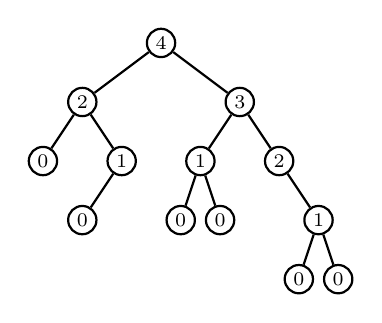
\begin{tikzpicture}
[-,thick,%
  every node/.style={shape=circle,inner sep=1.5pt,draw,thick},%
  scale=0.5]
\scriptsize
\node {$4$}
  [sibling distance=4cm]
  child {node {$2$}
    [sibling distance=2cm]
    child {node {$0$}}
    child {node {$1$}
      child {node {$0$}}
      child[missing]
    }
  }
  child {node {$3$}
    [sibling distance=2cm]
    child {node {$1$}
      [sibling distance=1cm]
      child {node {$0$}}
      child {node {$0$}}
    }
    child {node {$2$}
      child[missing]
      child {node {$1$}
        [sibling distance=1cm]
        child {node {$0$}}
        child {node {$0$}}
      }
    }
  };
\end{tikzpicture}
}
%%
%%
\qquad
\subfigure[Vertex inserted.]{
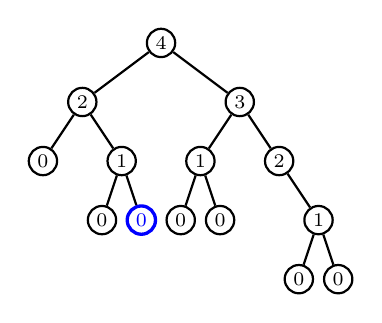
\begin{tikzpicture}
[-,thick,%
  every node/.style={shape=circle,inner sep=1.5pt,draw,thick},%
  scale=0.5]
\scriptsize
\node {$4$}
  [sibling distance=4cm]
  child {node {$2$}
    [sibling distance=2cm]
    child {node {$0$}}
    child {node {$1$}
      [sibling distance=1cm]
      child {node {$0$}}
      child {node[blue,very thick] {$0$}}
    }
  }
  child {node {$3$}
    [sibling distance=2cm]
    child {node {$1$}
      [sibling distance=1cm]
      child {node {$0$}}
      child {node {$0$}}
    }
    child {node {$2$}
      child[missing]
      child {node {$1$}
        [sibling distance=1cm]
        child {node {$0$}}
        child {node {$0$}}
      }
    }
  };
\end{tikzpicture}
}
%%
%%
\qquad
\subfigure[Vertex inserted.]{
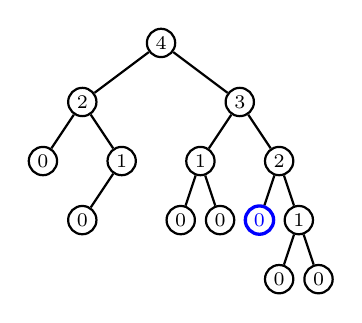
\begin{tikzpicture}
[-,thick,%
  every node/.style={shape=circle,inner sep=1.5pt,draw,thick},%
  scale=0.5]
\scriptsize
\node {$4$}
  [sibling distance=4cm]
  child {node {$2$}
    [sibling distance=2cm]
    child {node {$0$}}
    child {node {$1$}
      child {node {$0$}}
      child[missing]
    }
  }
  child {node {$3$}
    [sibling distance=2cm]
    child {node {$1$}
      [sibling distance=1cm]
      child {node {$0$}}
      child {node {$0$}}
    }
    child {node {$2$}
      [sibling distance=1cm]
      child {node[blue,very thick] {$0$}}
      child {node {$1$}
        [sibling distance=1cm]
        child {node {$0$}}
        child {node {$0$}}
      }
    }
  };
\end{tikzpicture}
}
\end{figure}

\end{document}
